%   ------------------------------------------------------------------------
\FloatBarrier
\section{CGDream}
\label{s.CGDreamApendice}

\begin{figure}[htbp]
    \centering
    \caption{\small Tela CGDream}
    \label{fig:CGDreamTela}
    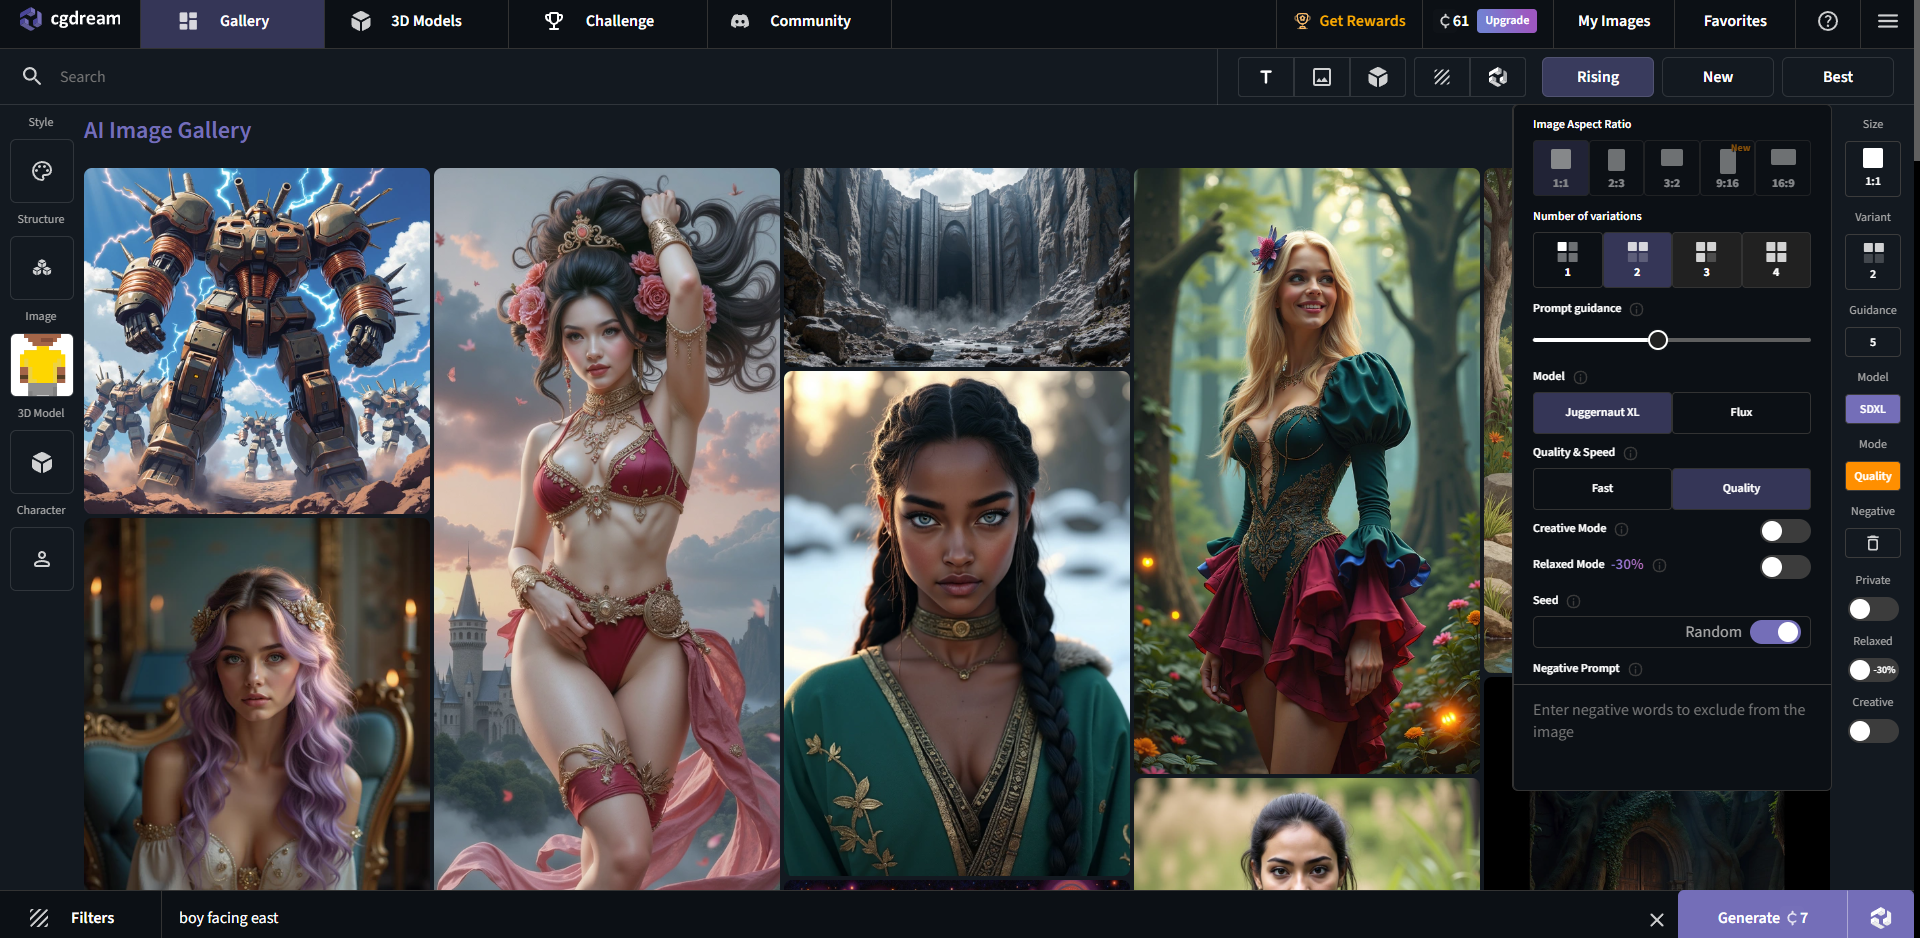
\includegraphics[width=1\linewidth]{figs/cgDream/tela_analise.png}
    \legend{\small Fonte: Elaborada pela autora.}
\end{figure}

\begin{figure}[htbp]
    \centering
    \caption{\small Opções de referência}
    \label{fig:CGDreamOpcoes}
    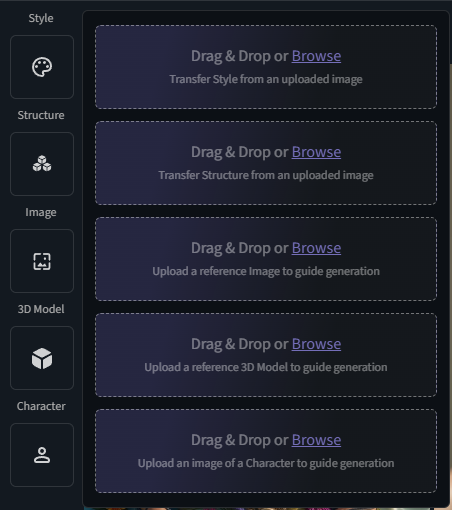
\includegraphics[width=0.4\linewidth]{figs/cgDream/tela_opcoes.PNG}
    \legend{\small Fonte: Elaborada pela autora.}
\end{figure}

\begin{figure}[htbp]
    \centering
    \caption{\small Processo da utilização 1 do CGDream (Imagem)}
    \label{fig:cgDream1}
    \begin{subfigure}{1\linewidth}
        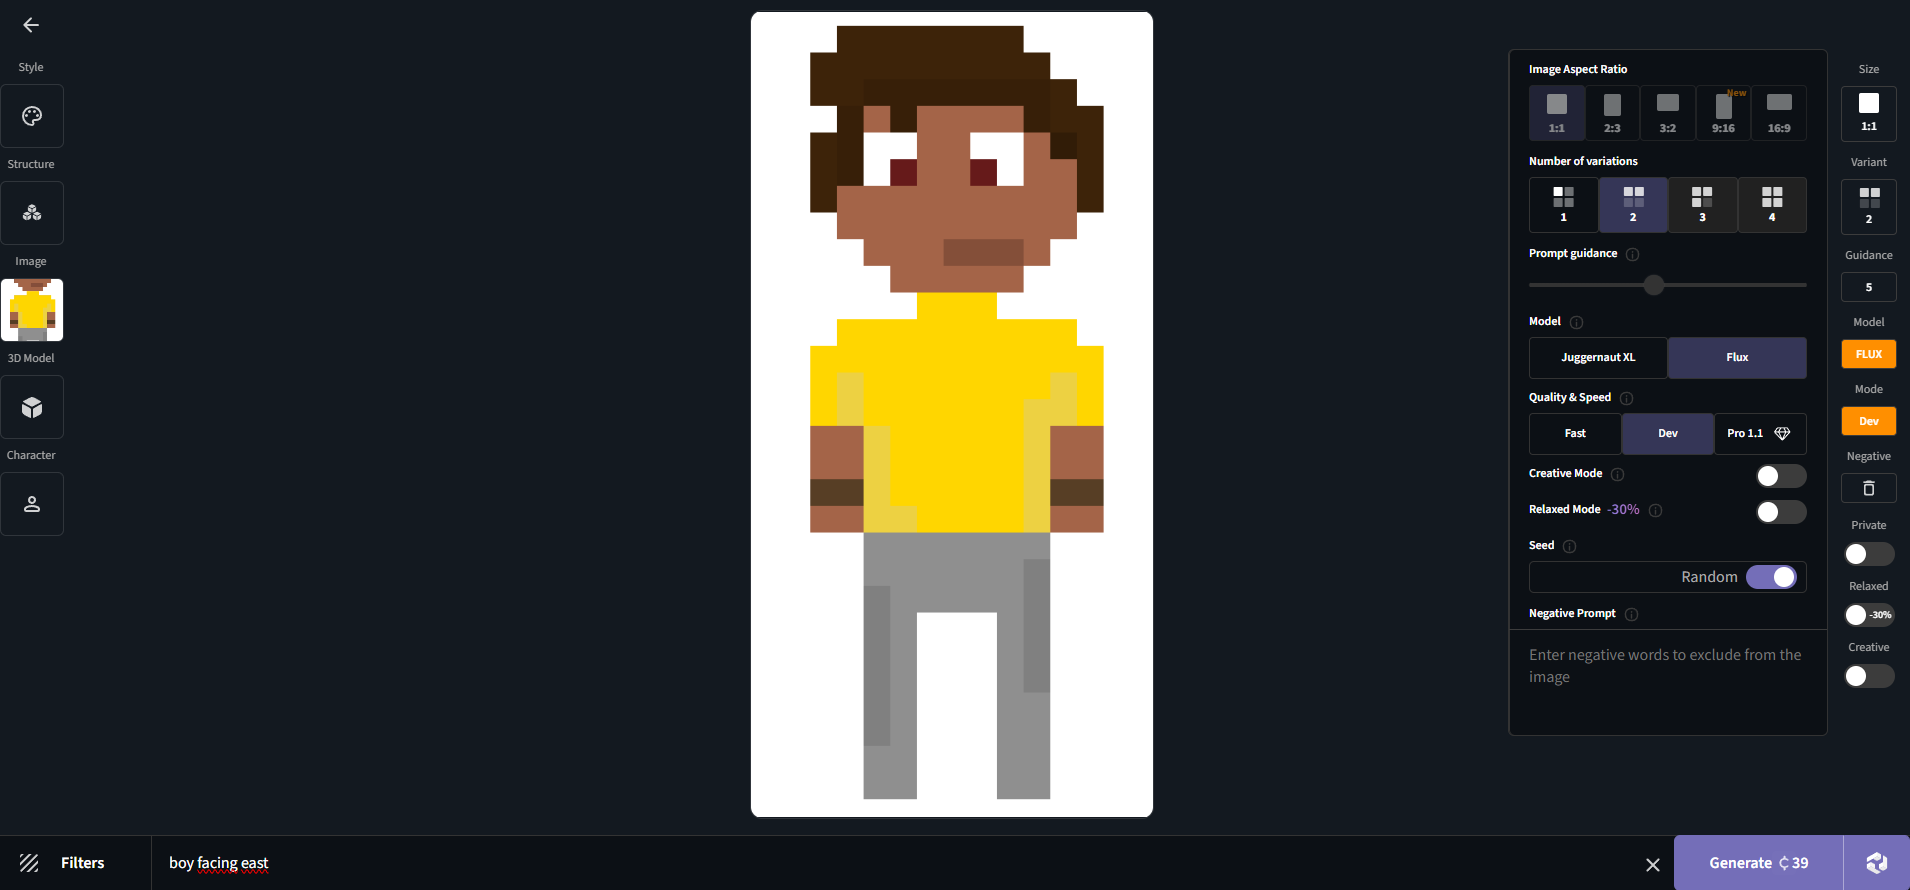
\includegraphics[width=1\linewidth]{figs/cgDream/tela_img_fluxDev.PNG}
        \caption{\small Selecionando modelo Flux, no modo Dev.}
        \label{fig:cgDream1a}
    \end{subfigure}
    \begin{subfigure}{0.25\linewidth}
        
\includegraphics[width=1\linewidth]{figs/cgDream/res_img_fluxDev1a.png}
        \caption{\small Imagem gerada 1.}
        \label{fig:cgDream1b}
    \end{subfigure}
    \begin{subfigure}{0.25\linewidth}
        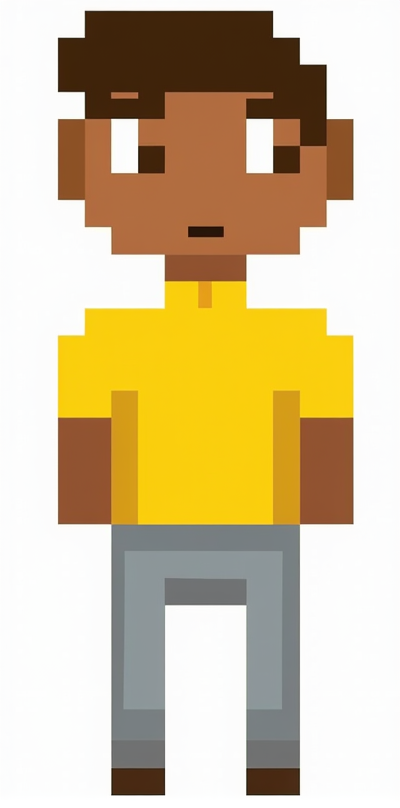
\includegraphics[width=1\linewidth]{figs/cgDream/res_img_fluxDev1b.png}
        \caption{\small Imagem gerada 2.}
        \label{fig:cgDream1c}
    \end{subfigure}
    \legend{\small Fonte: Elaborada pela autora.}
\end{figure}

\begin{figure}[htbp]
    \centering
    \caption{\small Processo da utilização 2 do CGDream (Imagem)}
    \label{fig:cgDream2}
    \begin{subfigure}{1\linewidth}
        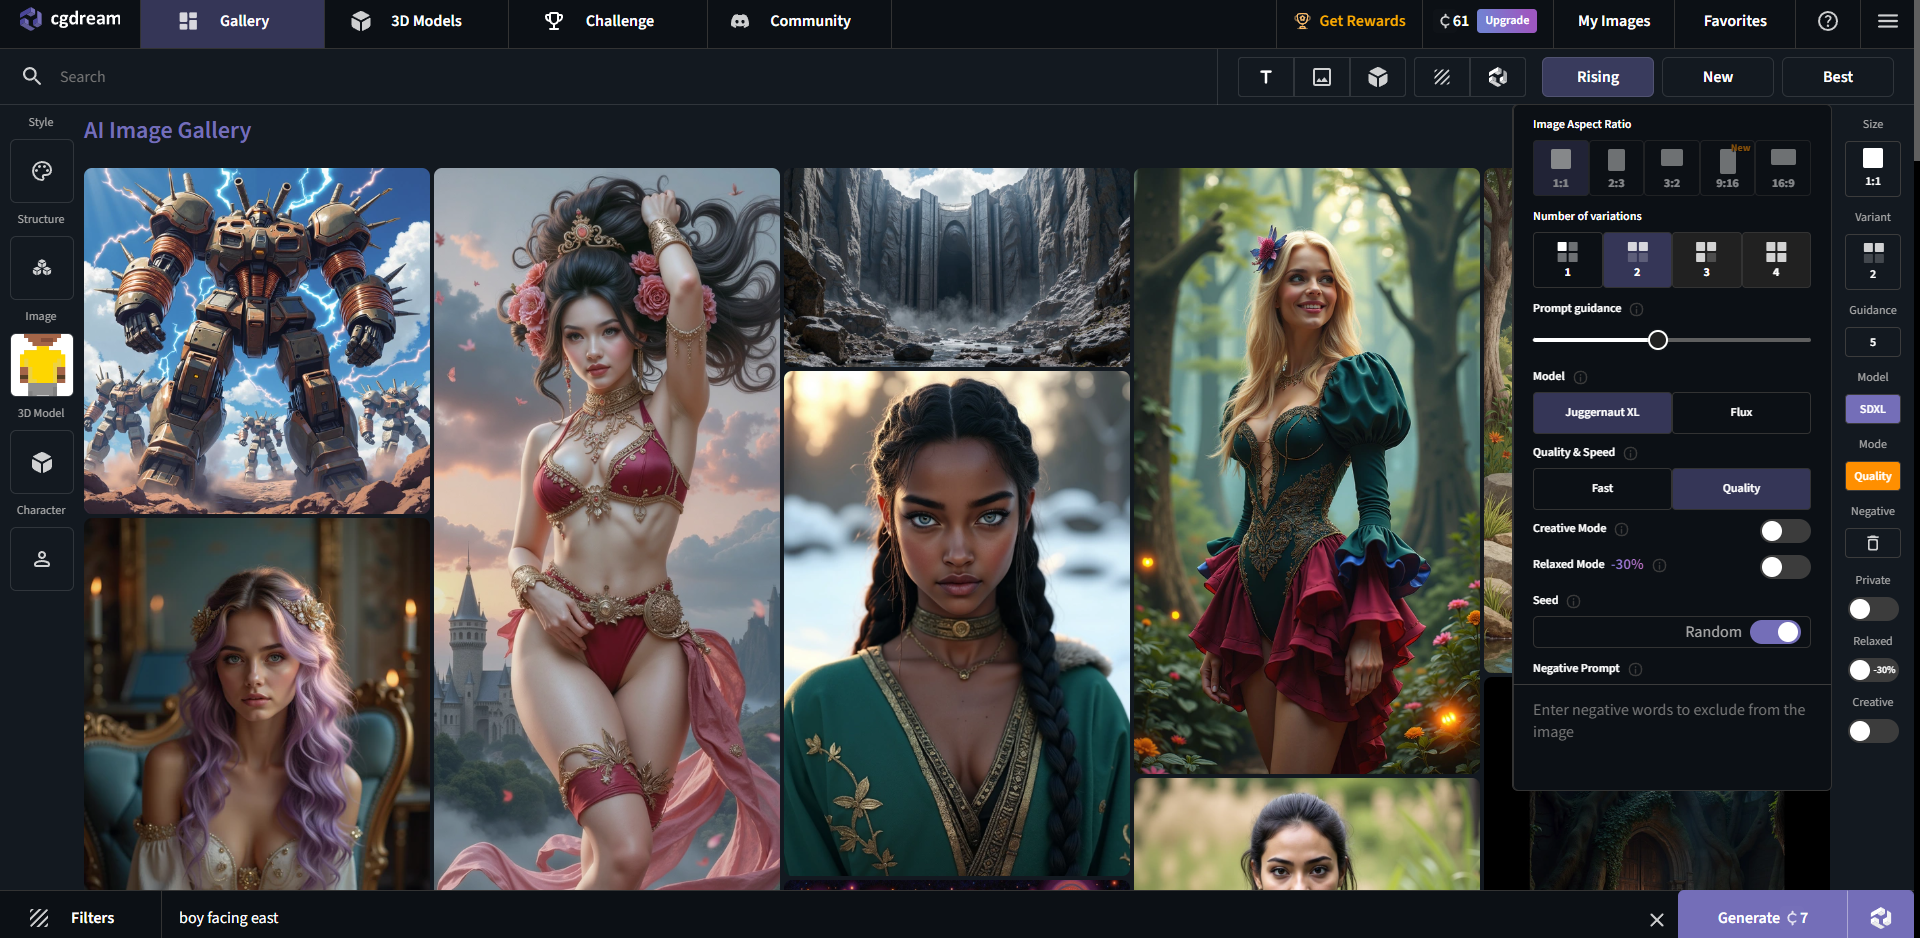
\includegraphics[width=1\linewidth]{figs/cgDream/tela_analise.png}
        \caption{\small Selecionando modelo Juggernaut XL, no modo Quality.}
        \label{fig:cgDream2a}
    \end{subfigure}
    \begin{subfigure}{0.15\linewidth}
        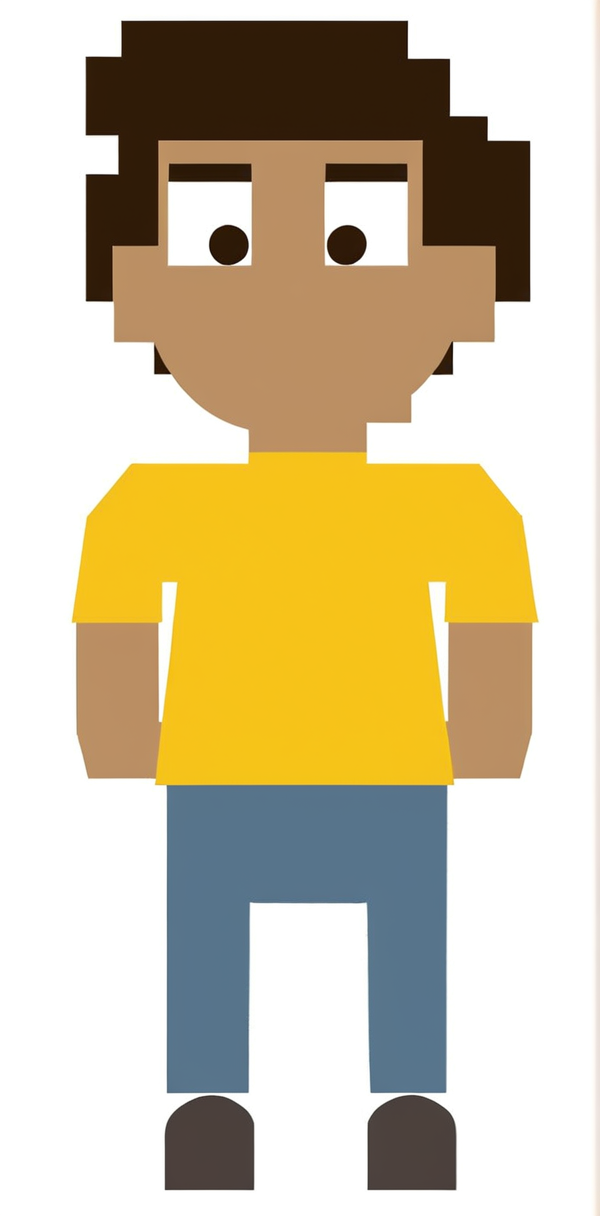
\includegraphics[width=1\linewidth]{figs/cgDream/res_img_jug2a.png}
        \caption{\small Imagem gerada 1.}
        \label{fig:cgDream2b}
    \end{subfigure}
    \begin{subfigure}{0.15\linewidth}
        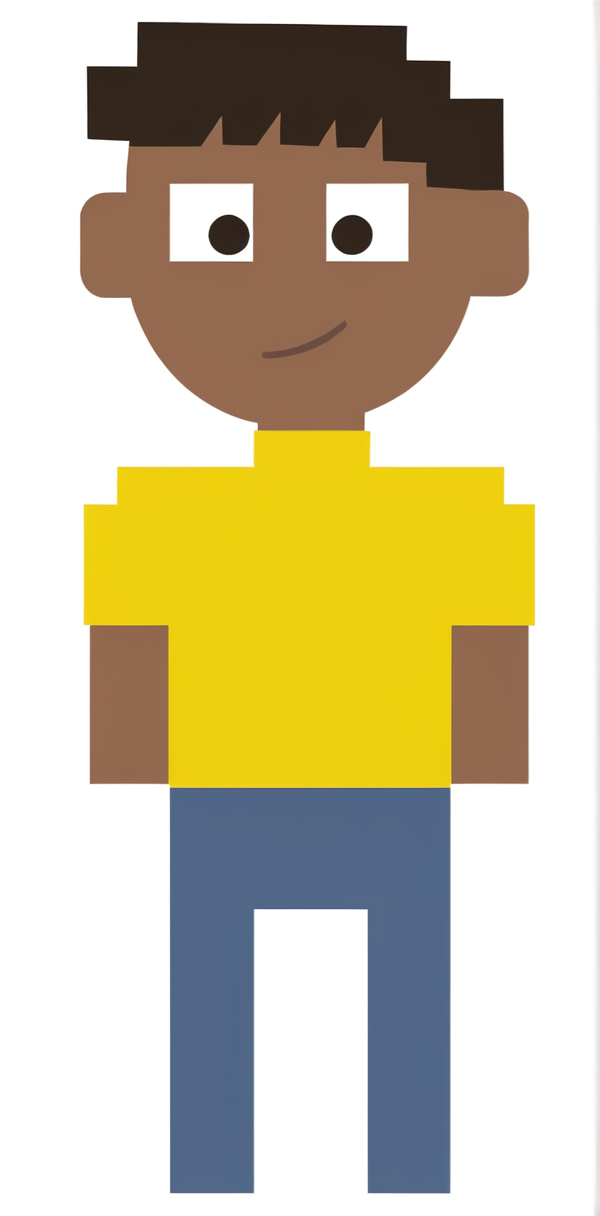
\includegraphics[width=1\linewidth]{figs/cgDream/res_img_jug2b.png}
        \caption{\small Imagem gerada 2.}
        \label{fig:cgDream2c}
    \end{subfigure}
    \legend{\small Fonte: Elaborada pela autora, utilizando a ferramenta CGDream.}
\end{figure}

\begin{figure}[htbp]
    \centering
    \caption{\small Resultado do modelo Juggernaut XL com prompt guidance em 8}
    \label{fig:cgDreamJugger8}
    \begin{subfigure}{0.15\linewidth}
        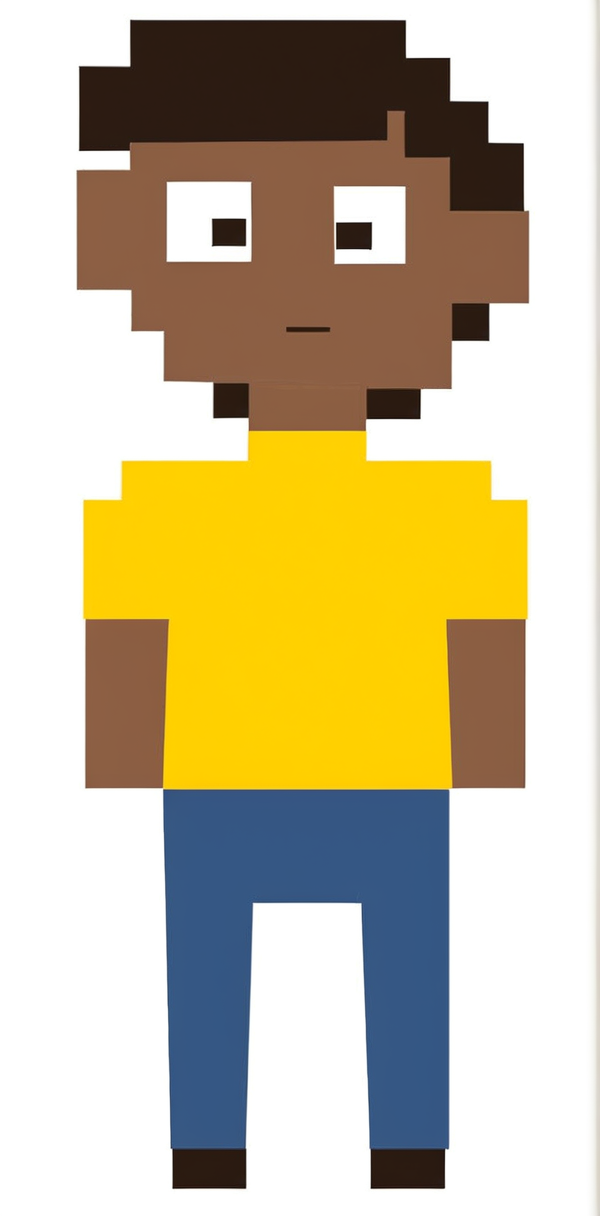
\includegraphics[width=1\linewidth]{figs/cgDream/res_img_jug8a.png}
        \caption{\small Imagem gerada 1.}
        \label{fig:cgDreamJugger8a}
    \end{subfigure}
    \begin{subfigure}{0.15\linewidth}
        
\includegraphics[width=1\linewidth]{figs/cgDream/res_img_jug8b.png}
        \caption{\small Imagem gerada 2.}
        \label{fig:cgDreamJugger8b}
    \end{subfigure}
    \legend{\small Fonte: Elaborada pela autora, utilizando a ferramenta CGDream.}
\end{figure}

\begin{figure}[htbp]
    \centering
    \caption{\small Processo da utilização 3 do CGDream (Imagem)}
    \label{fig:cgDream3}
    \begin{subfigure}{0.9\linewidth}
        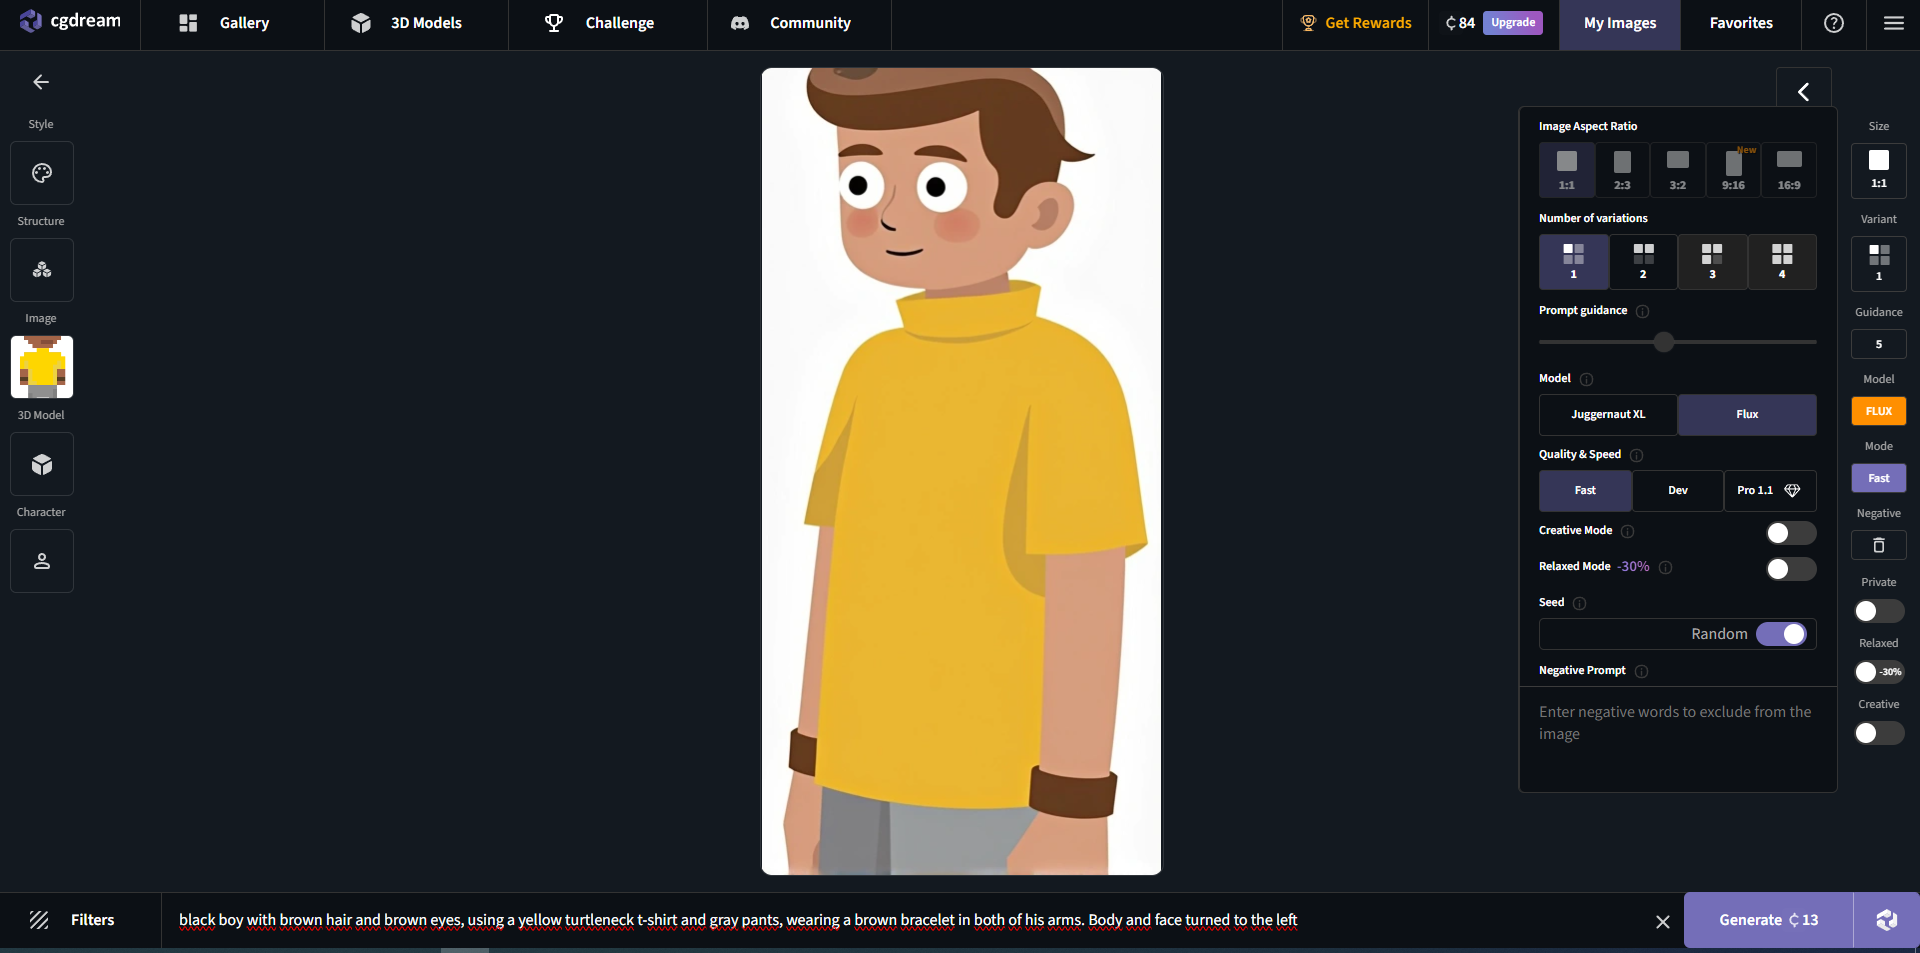
\includegraphics[width=1\linewidth]{figs/cgDream/tela_img_FluxFast1.PNG}
        \caption{\small Selecionando modelo Flux, no modo Fast.}
        \label{fig:cgDream3a}
    \end{subfigure}
    \begin{subfigure}{0.15\linewidth}
        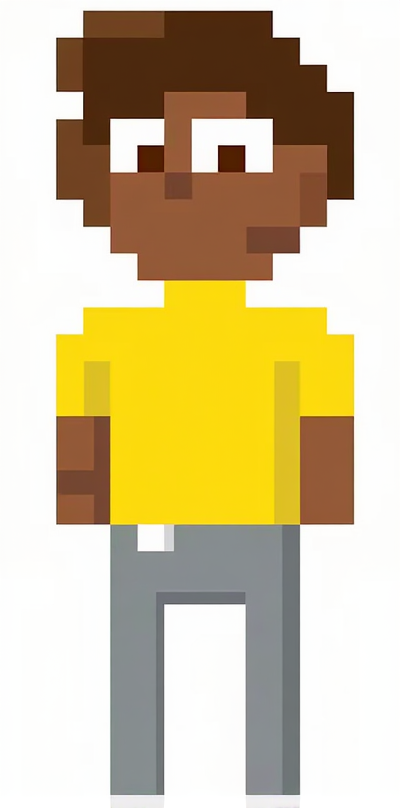
\includegraphics[width=1\linewidth]{figs/cgDream/res_img_FluxFast1a.png}
        \caption{\small Imagem gerada 1.}
        \label{fig:cgDream3b}
    \end{subfigure}
    \begin{subfigure}{0.15\linewidth}
        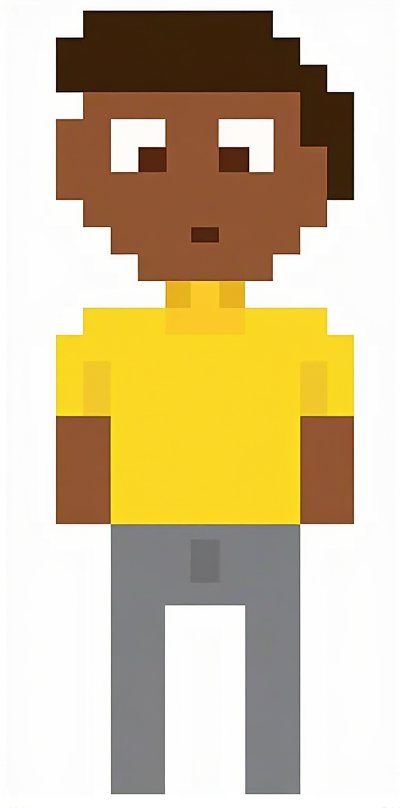
\includegraphics[width=1\linewidth]{figs/cgDream/res_img_FluxFast1b.png}
        \caption{\small Imagem gerada 2.}
        \label{fig:cgDream3c}
    \end{subfigure}
    \begin{subfigure}{1\linewidth}
        
\includegraphics[width=1\linewidth]{figs/cgDream/tela_img_FluxFast2.PNG}
        \caption{\small Novo teste de prompt no modelo Flux.}
        \label{fig:cgDream3d}
    \end{subfigure}
    \begin{subfigure}{0.2\linewidth}
        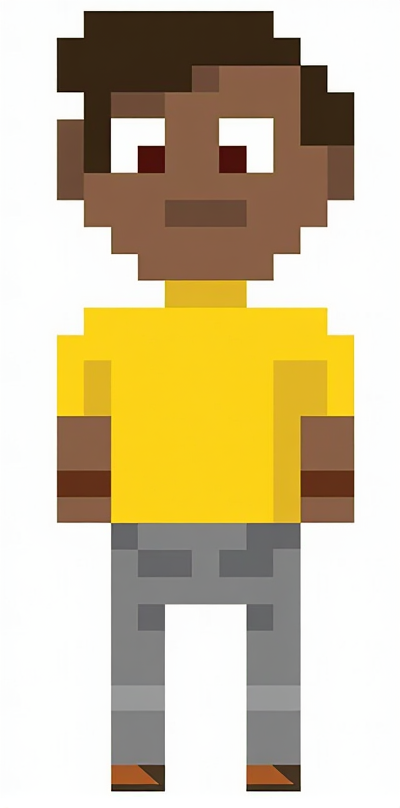
\includegraphics[width=1\linewidth]{figs/cgDream/res_img_FluxFast2.png}
        \caption{\small Imagem gerada pelo modo Fast.}
        \label{fig:cgDream3e}
    \end{subfigure}
    \begin{subfigure}{0.2\linewidth}
        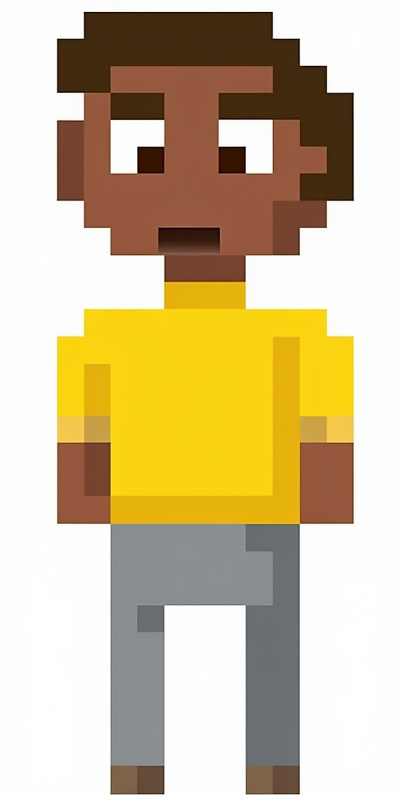
\includegraphics[width=1\linewidth]{figs/cgDream/res_img_FluxDev2.png}
        \caption{\small Imagem gerada pelo modo Dev.}
        \label{fig:cgDream3f}
    \end{subfigure}
    \legend{\small Fonte: Elaborada pela autora, utilizando a ferramenta CGDream.}
\end{figure}

\begin{figure}[htbp]
    \centering
    \caption{\small Processo da utilização 4 do CGDream (Imagem)}
    \label{fig:cgDream4}
    \begin{subfigure}{0.9\linewidth}
        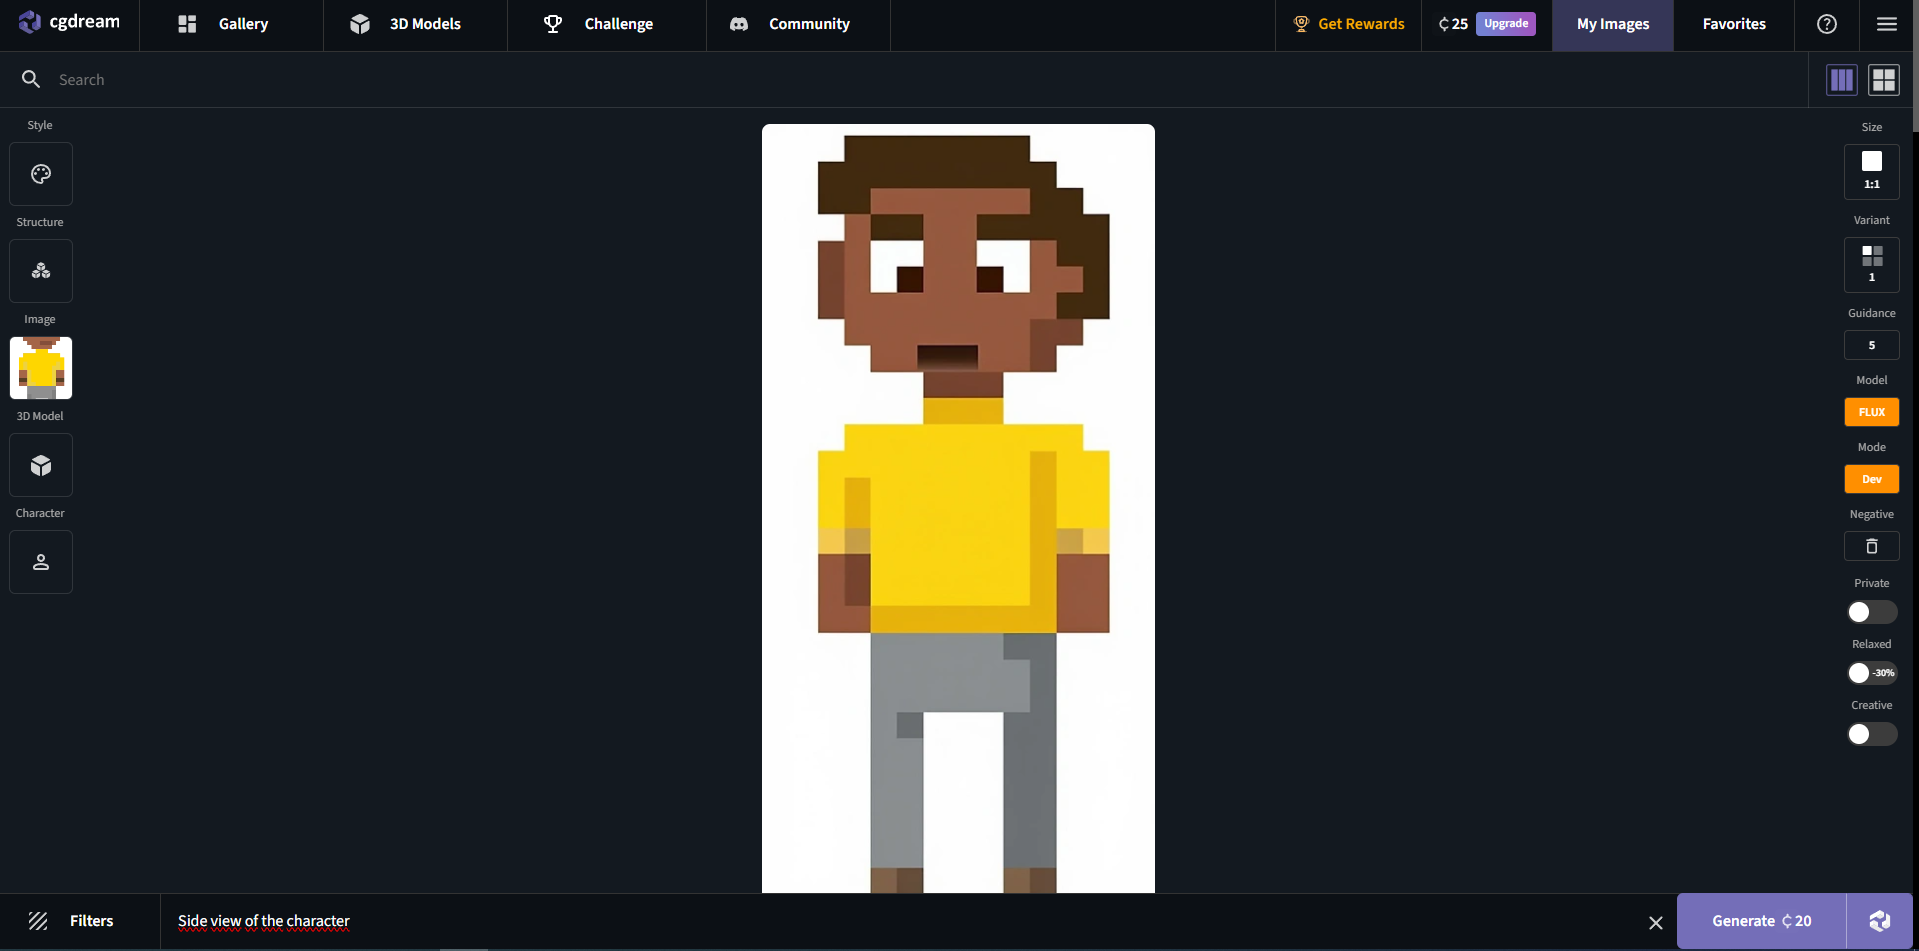
\includegraphics[width=1\linewidth]{figs/cgDream/tela_img_FluxDev3.PNG}
        \caption{\small Selecionando modelo Flux, no modo Dev.}
        \label{fig:cgDream4a}
    \end{subfigure}
    \begin{subfigure}{0.15\linewidth}
        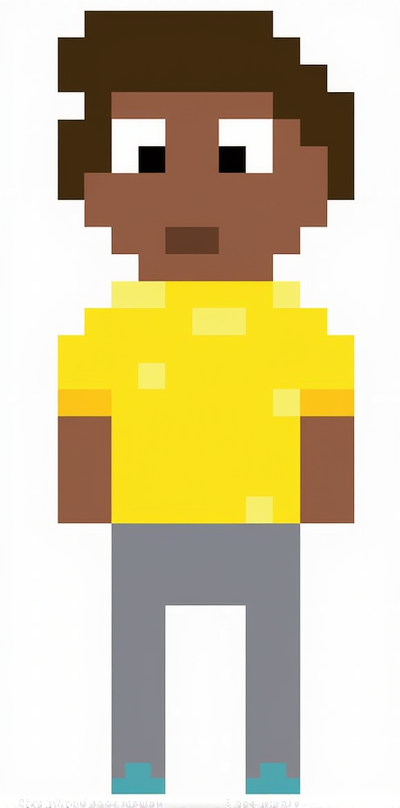
\includegraphics[width=1\linewidth]{figs/cgDream/res_img_FluxDev3.png}
        \caption{\small Imagem gerada.}
        \label{fig:cgDream4b}
    \end{subfigure}
    \legend{\small Fonte: Elaborada pela autora, utilizando a ferramenta CGDream.}
\end{figure}


\begin{figure}[htbp]
    \centering
    \caption{\small Processo da utilização 5 do CGDream (Personagem)}
    \label{fig:cgDream5}
    \begin{subfigure}{0.9\linewidth}
        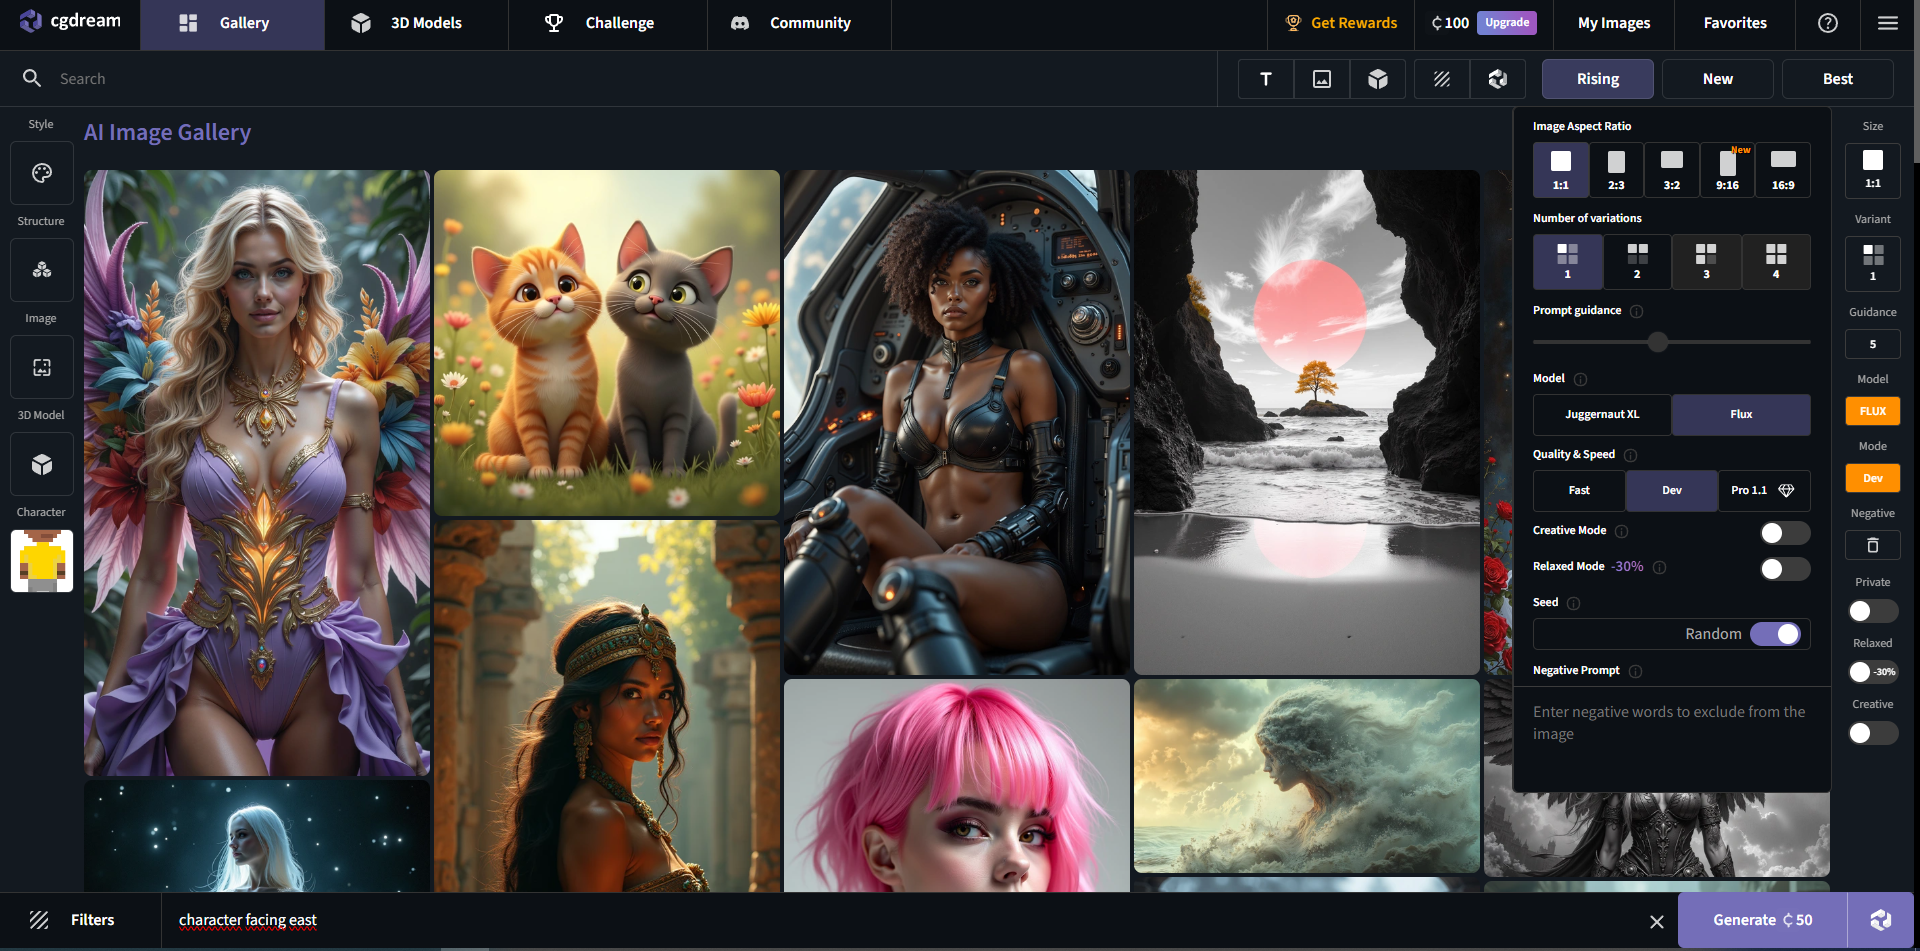
\includegraphics[width=1\linewidth]{figs/cgDream/tela_char_FluxDev1.png}
        \caption{\small Selecionando modelo Flux, no modo Dev.}
        \label{fig:cgDream5a}
    \end{subfigure}
    \begin{subfigure}{0.7\linewidth}
        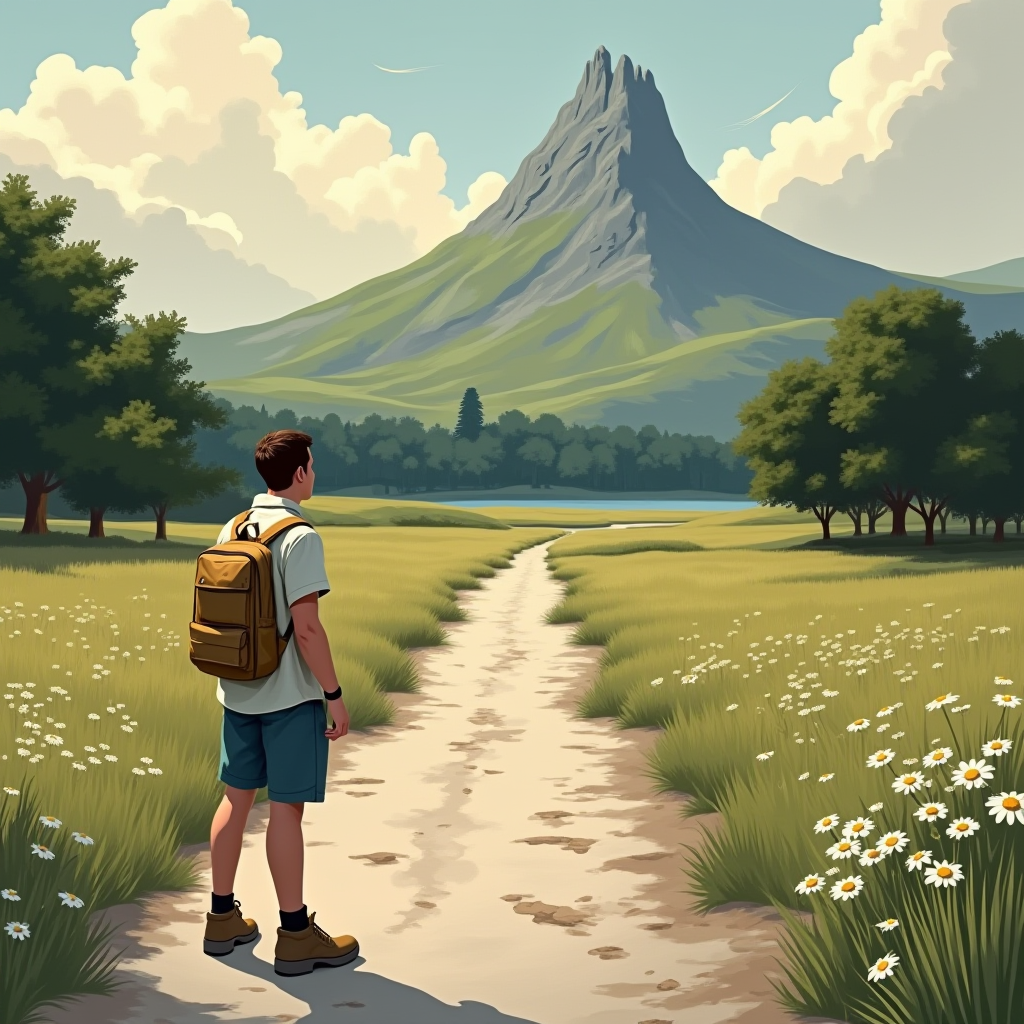
\includegraphics[width=1\linewidth]{figs/cgDream/res_char_FluxDev1.png}
        \caption{\small Imagem gerada.}
        \label{fig:cgDream5b}
    \end{subfigure}
    \legend{\small Fonte: Elaborada pela autora, utilizando a ferramenta CGDream.}
\end{figure}

\begin{figure}[htbp]
    \centering
    \caption{\small Processo da utilização 6 do CGDream (Personagem)}
    \label{fig:cgDream6}
    \begin{subfigure}{0.45\linewidth}
        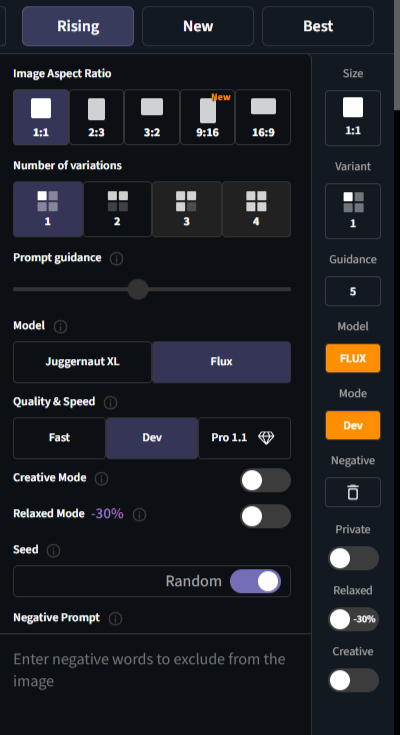
\includegraphics[width=1\linewidth]{figs/cgDream/tela_char_Jug9_1.png}
        \caption{\small Selecionando modelo Juggernaut XL, no modo Quality com prompt guidance em 9.}
        \label{fig:cgDream6a}
    \end{subfigure}
    \begin{subfigure}{0.45\linewidth}
        \centering
        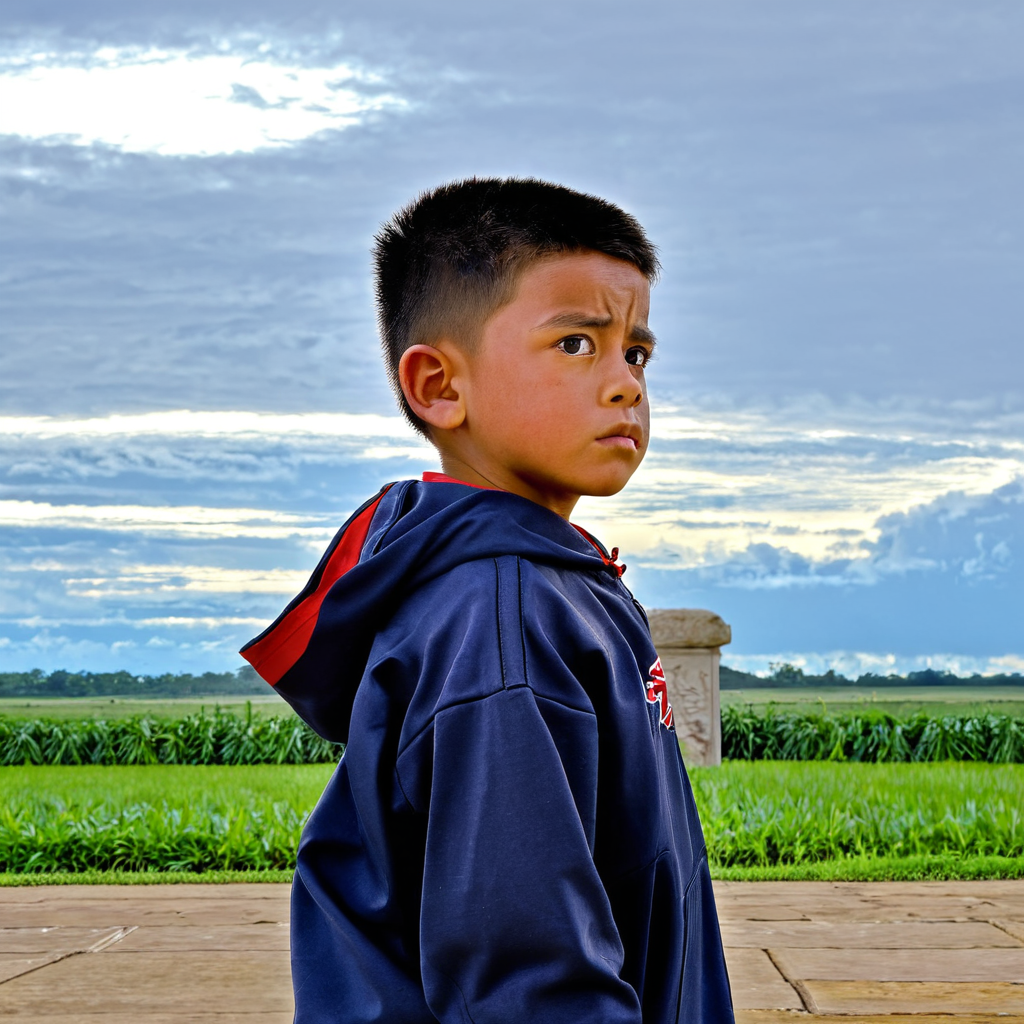
\includegraphics[width=1\linewidth]{figs/cgDream/res_char_Jug9_1.png}
        \caption{\small Imagem gerada.}
        \label{fig:cgDream6b}
    \end{subfigure}
    \legend{\small Fonte: Elaborada pela autora, utilizando a ferramenta CGDream.}
\end{figure}

\begin{figure}[htbp]
    \centering
    \caption{\small Processo da utilização 7 do CGDream (Personagem)}
    \label{fig:cgDream7}
    \begin{subfigure}{1\linewidth}
        
\includegraphics[width=1\linewidth]{figs/cgDream/tela_prompt_char.PNG}
        \caption{\small Prompt.}
        \label{fig:cgDream7a}
    \end{subfigure}
    \begin{subfigure}{0.45\linewidth}
        \centering
        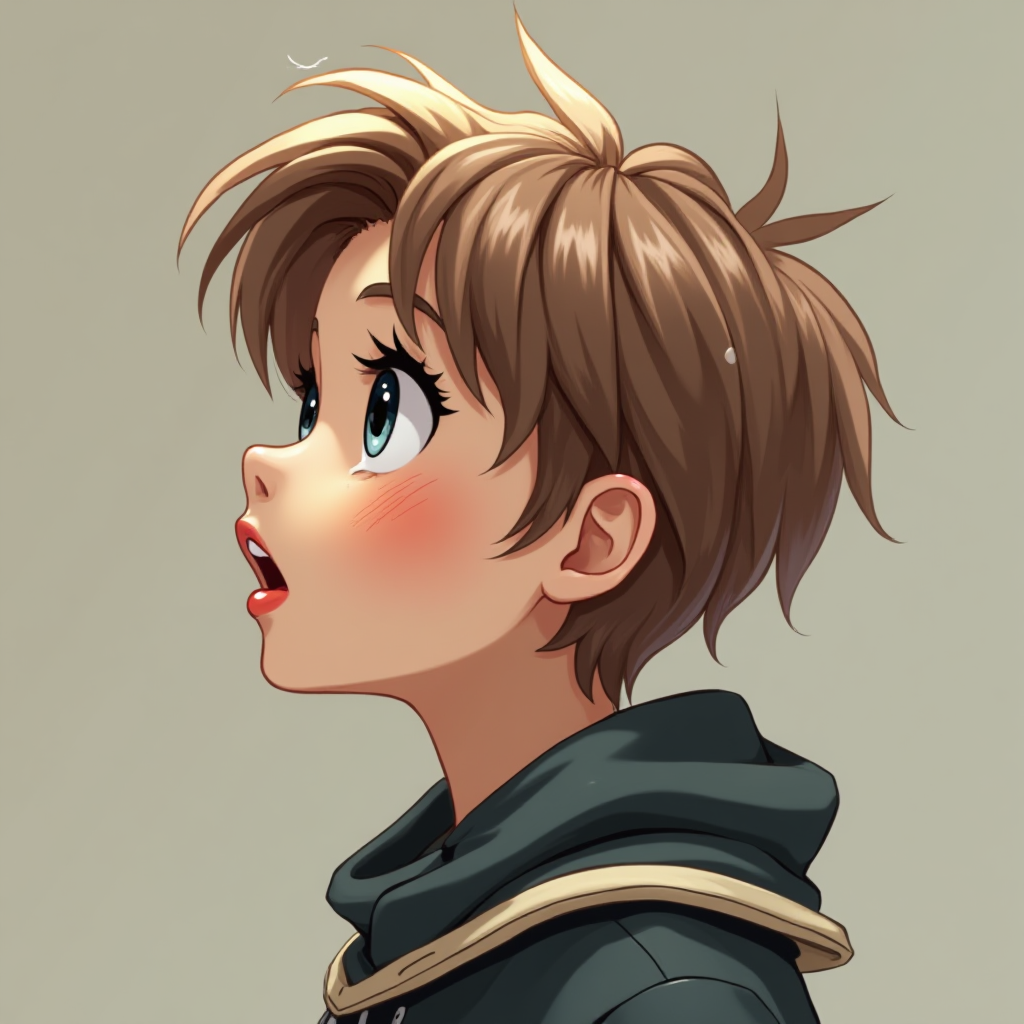
\includegraphics[width=1\linewidth]{figs/cgDream/res_char_fluxFast1.png}
        \caption{\small Imagem gerada pelo modelo Flux no modo Fast.}
        \label{fig:cgDream7b}
    \end{subfigure}
    \begin{subfigure}{0.45\linewidth}
        \centering
        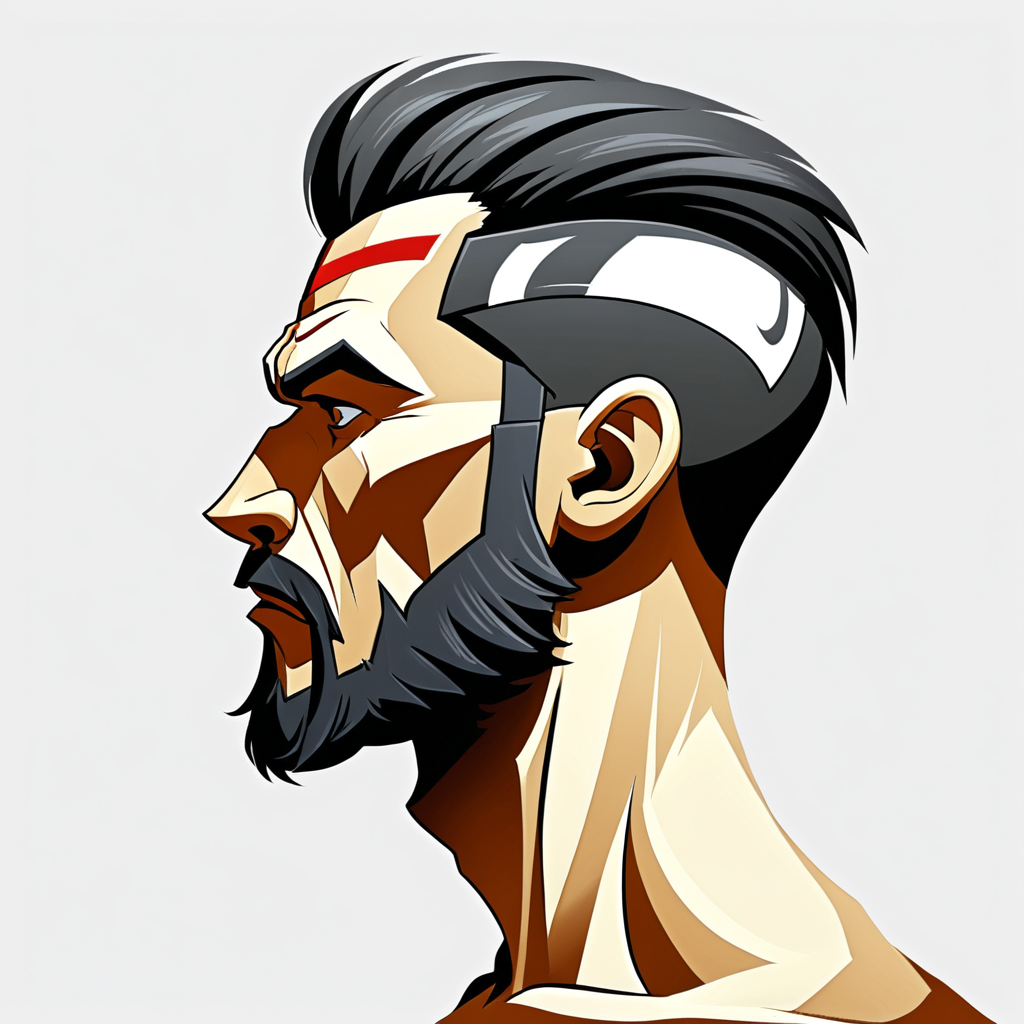
\includegraphics[width=1\linewidth]{figs/cgDream/res_char_jug8.png}
        \caption{\small Imagem gerada pelo modelo Juggernaut XL no modo Quality com prompt guidance em 8 e "3D" como palavra negativa.}
        \label{fig:cgDream7c}
    \end{subfigure}
    \legend{\small Fonte: Elaborada pela autora, utilizando a ferramenta CGDream.}
\end{figure}

\begin{figure}[htbp]
    \centering
    \caption{\small Processo da utilização 8 do CGDream (Personagem)}
    \label{fig:cgDream8}
    \begin{subfigure}{0.7\linewidth}
        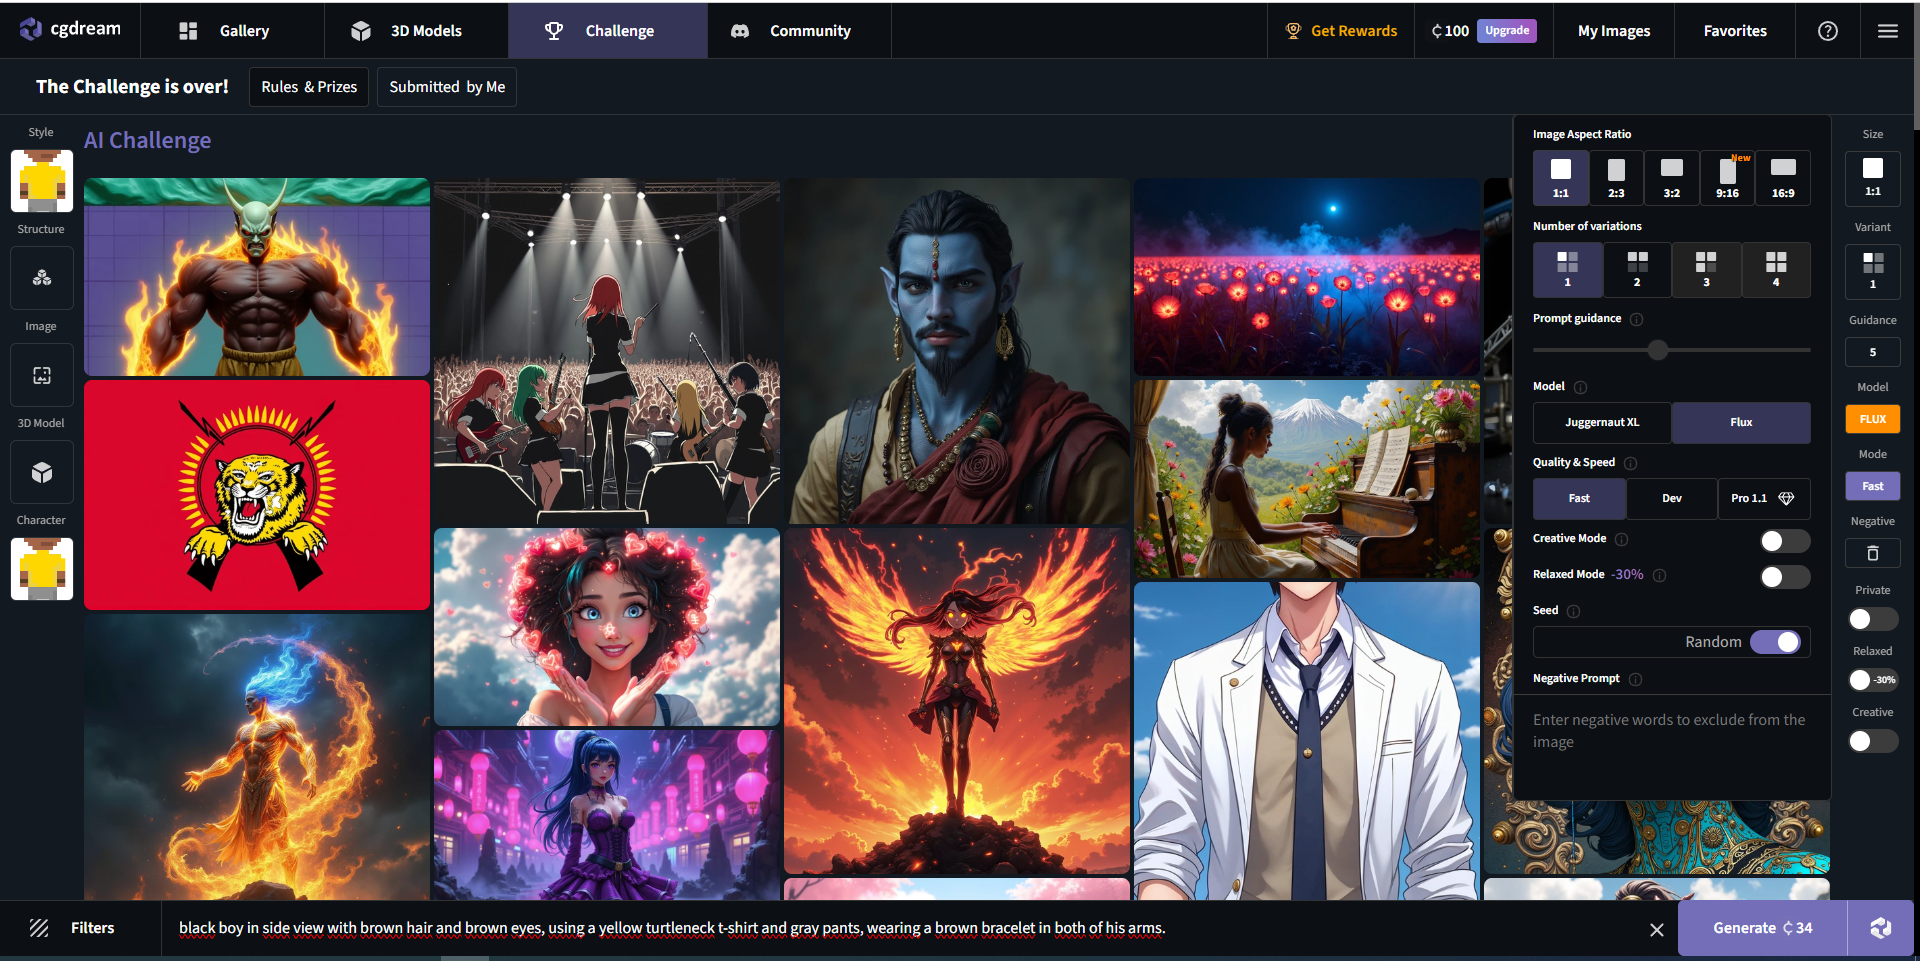
\includegraphics[width=1\linewidth]{figs/cgDream/tela_char_FluxFast_estilo.PNG}
        \caption{\small Estilo de referência e prompt.}
        \label{fig:cgDream8a}
    \end{subfigure}
    \begin{subfigure}{0.35\linewidth}
        \centering
        
\includegraphics[width=1\linewidth]{figs/cgDream/res_char_FluxFast_estilo1.png}
        \caption{\small Imagem gerada pelo modelo Flux no modo Fast.}
        \label{fig:cgDream8b}
    \end{subfigure}
    \begin{subfigure}{0.35\linewidth}
        \centering
        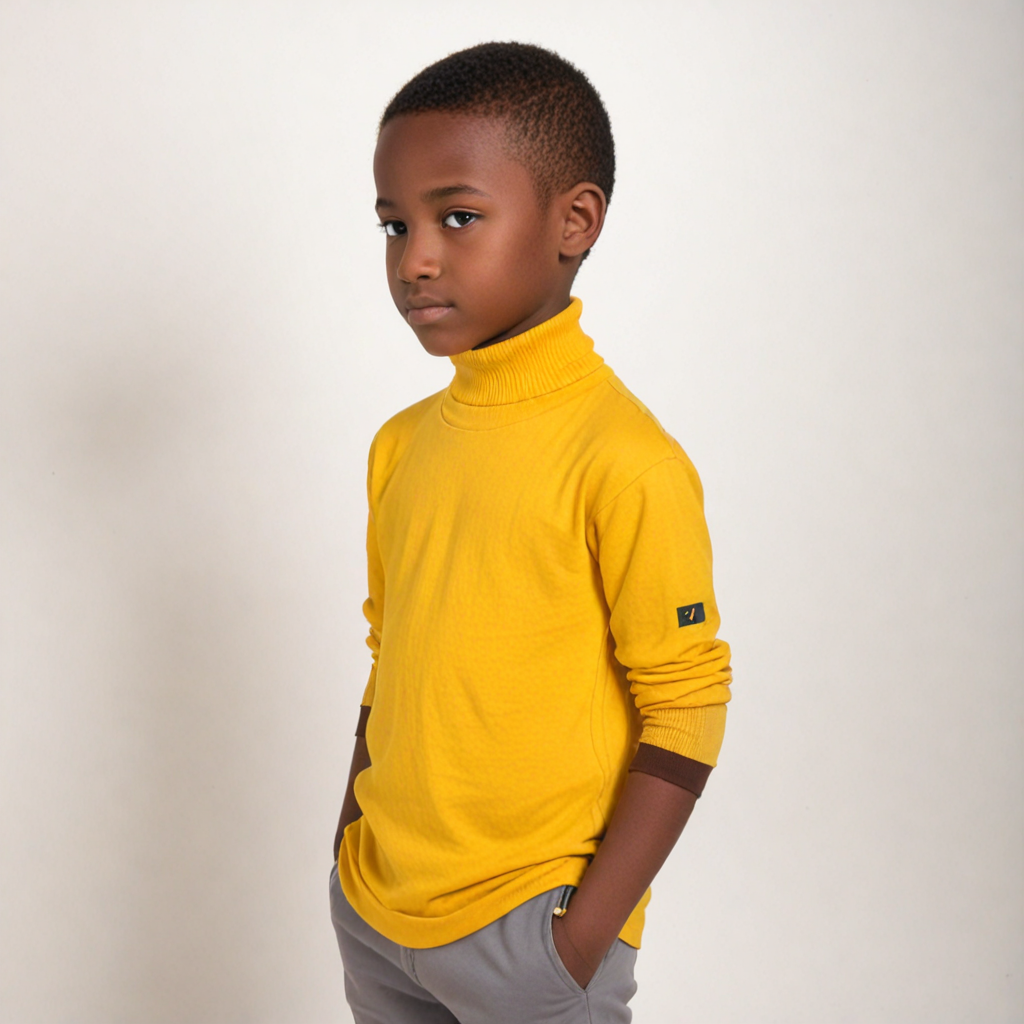
\includegraphics[width=1\linewidth]{figs/cgDream/res_char_jug_estilo1a.png}
        \caption{\small Imagem gerada pelo modelo Juggernaut XL no modo Fast com "blur" (borrão, em inglês) como palavra negativa.}
        \label{fig:cgDream8c}
    \end{subfigure}
    \begin{subfigure}{0.35\linewidth}
        \centering
        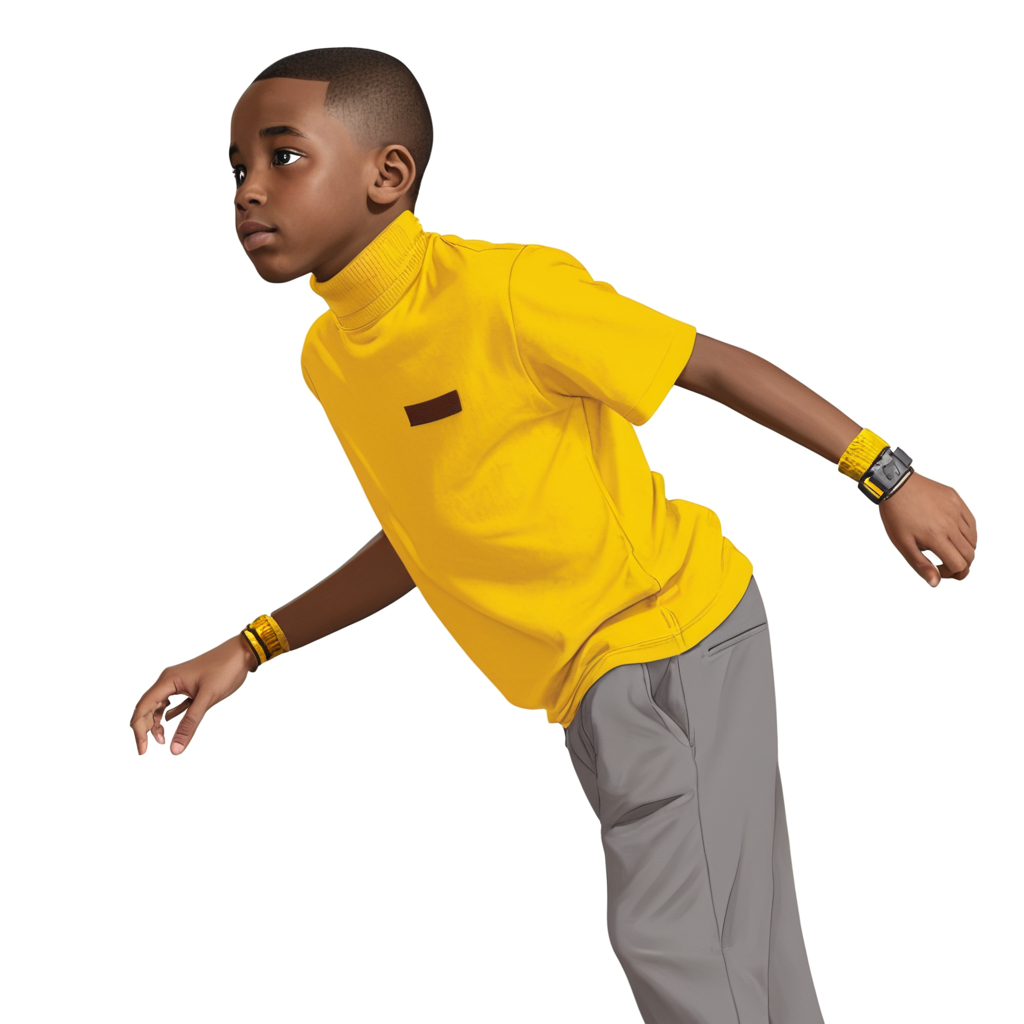
\includegraphics[width=1\linewidth]{figs/cgDream/res_char_jug_estilo1b.png}
        \caption{\small Imagem gerada pelo modelo Juggernaut XL no modo Quality com blur como palavra negativa.}
        \label{fig:cgDream8d}
    \end{subfigure}
    \begin{subfigure}{0.35\linewidth}
        \centering
        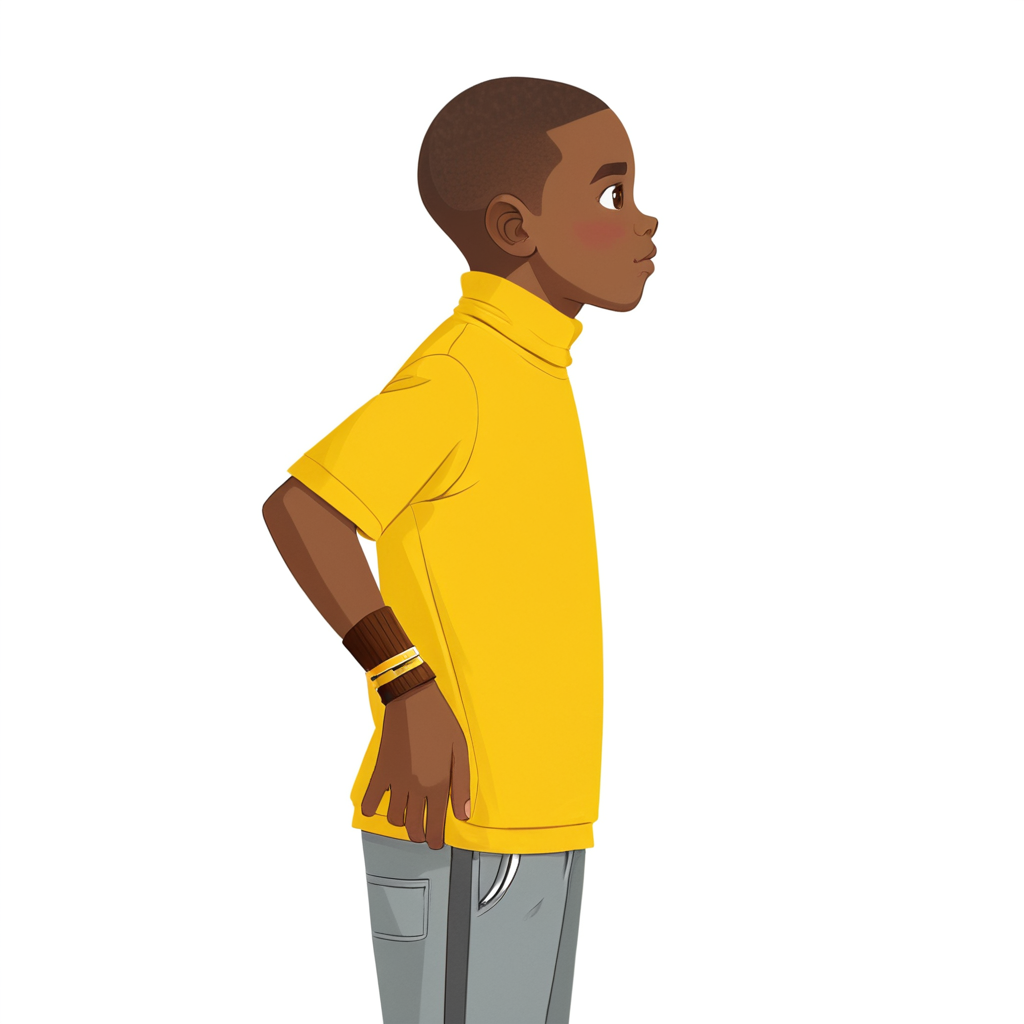
\includegraphics[width=1\linewidth]{figs/cgDream/res_char_jug_estilo1c.png}
        \caption{\small Imagem gerada pelo modelo Juggernaut XL no modo Quality com "blur" e "3D" como palavra negativa.}
        \label{fig:cgDream8e}
    \end{subfigure}
    \legend{\small Fonte: Elaborada pela autora, utilizando a ferramenta CGDream.}
\end{figure}

\begin{figure}[htbp]
    \centering
    \caption{\small Processo da utilização 9 do CGDream (Personagem)}
    \label{fig:cgDream9}
    \begin{subfigure}{0.7\linewidth}
        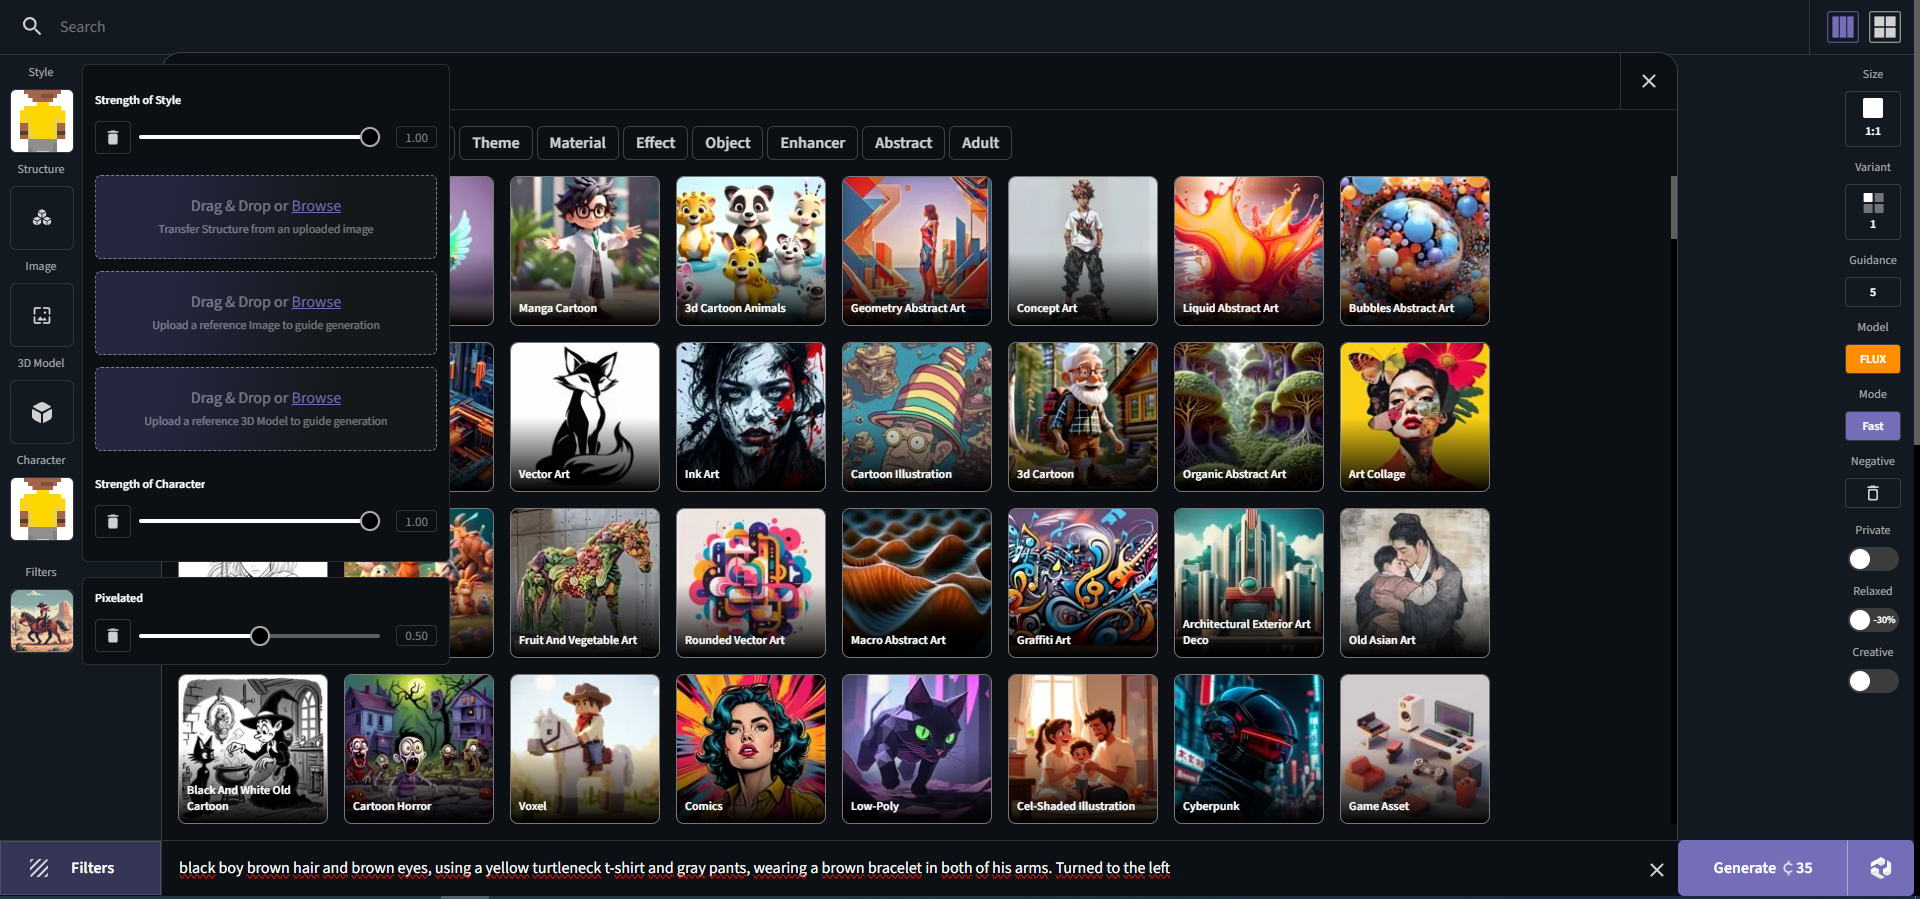
\includegraphics[width=1\linewidth]{figs/cgDream/tela_char_FluxFast_filtro1.PNG}
        \caption{\small Selecionando modelo Flux, no modo Fast com filtro de pixel.}
        \label{fig:cgDream9a}
    \end{subfigure}
    \begin{subfigure}{0.35\linewidth}
        \centering
        
\includegraphics[width=1\linewidth]{figs/cgDream/res_char_FluxFast_filtro1.png}
        \caption{\small Imagem gerada.}
        \label{fig:cgDream9b}
    \end{subfigure}
    \begin{subfigure}{0.35\linewidth}
        \centering
        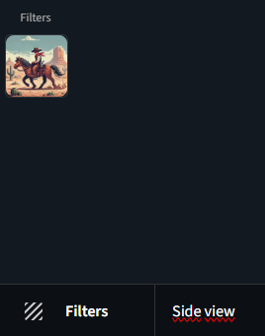
\includegraphics[width=1\linewidth]{figs/cgDream/tela_char_FluxFast_filtro2.PNG}
        \caption{\small Prompt simples.}
        \label{fig:cgDream9c}
    \end{subfigure}
    \begin{subfigure}{0.45\linewidth}
        \centering
        
\includegraphics[width=1\linewidth]{figs/cgDream/res_char_FluxFast_filtro2.PNG}
        \caption{\small Imagem gerada pelo prompt simples.}
        \label{fig:cgDream9d}
    \end{subfigure}


    \legend{\small Fonte: Elaborada pela autora, utilizando a ferramenta CGDream.}
\end{figure}